\section{Step API}

\begin{figure}
	\centering
	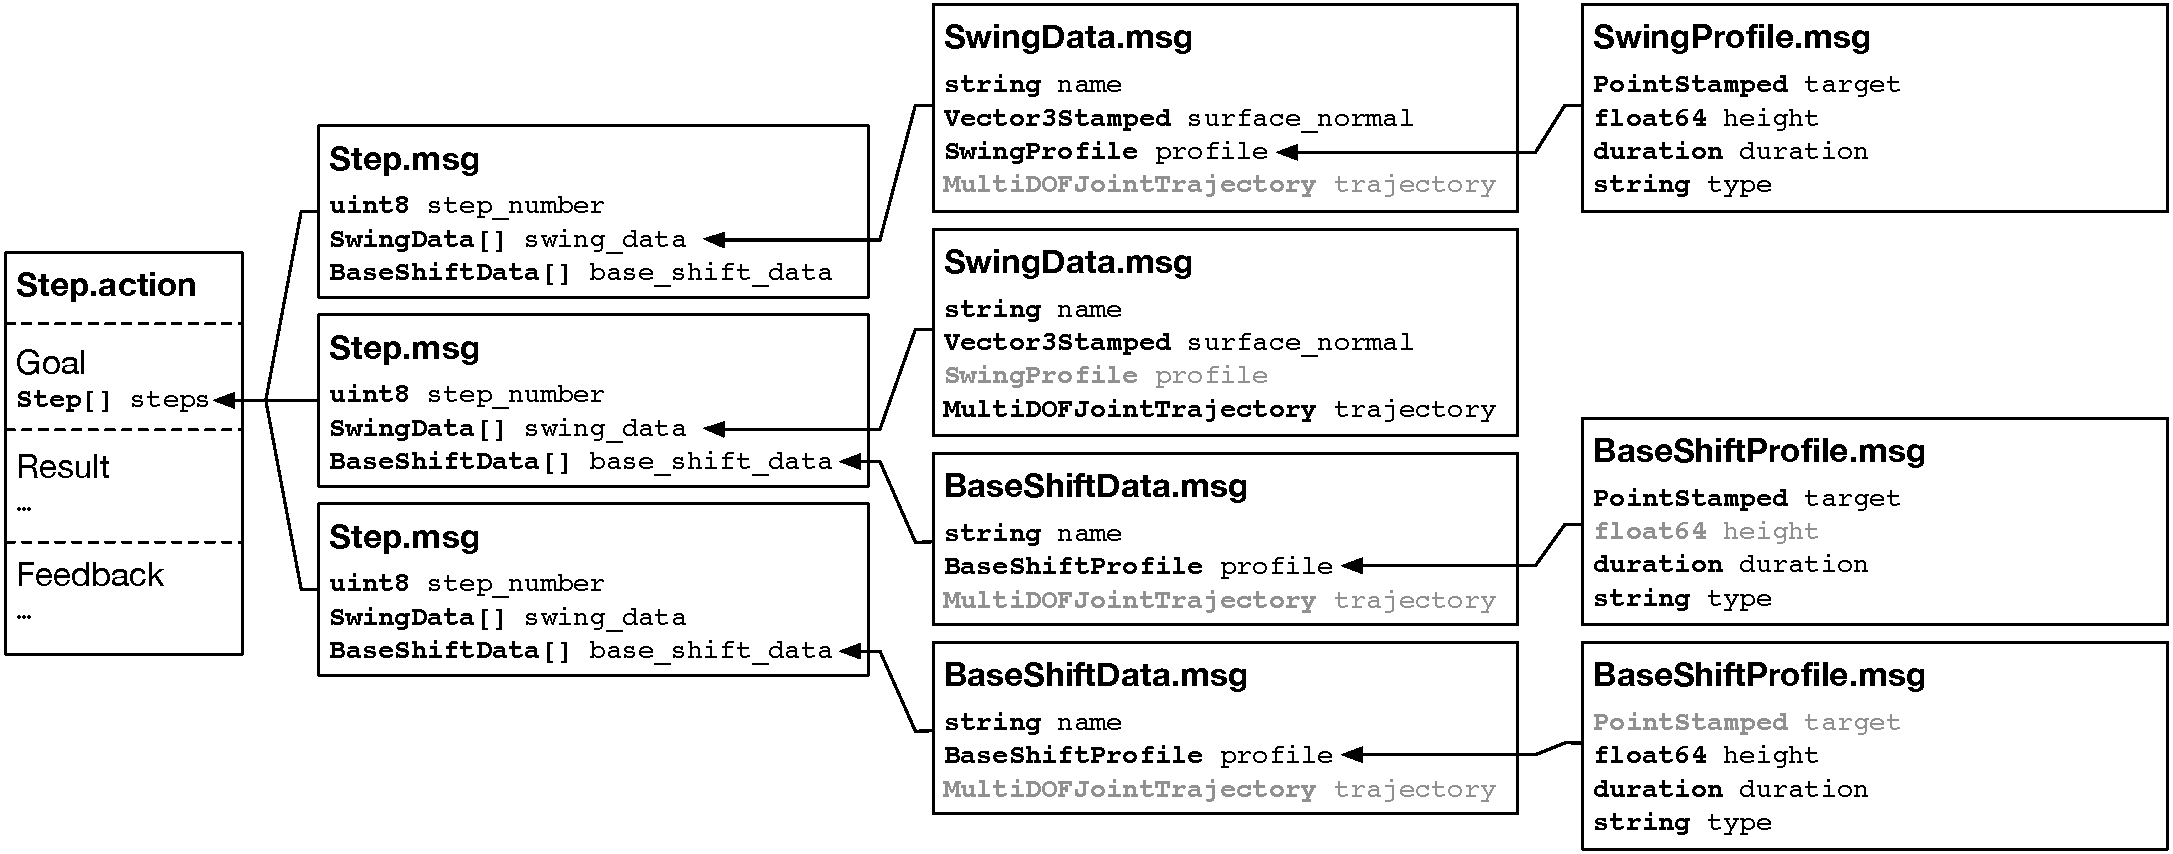
\includegraphics[width=1.0 \textwidth]{images/step_api_structure} 
	\caption{Step API Structure}
	\label{fig:step_api_structure}
\end{figure}

\begin{code}
# Step.msg

# The step number starting from 1, monotonically increasing during
# action, resets to 1 if robot leaves action.
uint8 step_number

# Swing data for each swing leg.
starleth_msgs/SwingData[] swing_data

# Base shift data for different states of the step.
starleth_msgs/BaseShiftData[] shift_data
\end{code}

\begin{code}
# Step.action Goal

starleth_msgs/Step[] steps
\end{code}

\begin{code}
# SwingData.msg
# Representation of swing data for one leg.

# Leg type identifiers ('leftFore', 'rightHind' etc.).
string name

# Target foothold surface normal (if [0, 0, 0] set to [0, 0, 1] in world frame).
geometry_msgs/Vector3Stamped surface_normal

# Either: Define a profile for the foot.
starleth_msgs/SwingProfile profile

# Or: Define the entire swing trajectory for the foot.
# The trajectory is used if it contains data, otherwise the profile is used.
trajectory_msgs/MultiDOFJointTrajectory trajectory	
\end{code}

\begin{code}
# SwingProfile.msg
# Definition of a swing leg profile.

# Target position of the foot by the end of the profile.
geometry_msgs/PointStamped target

# Step apex swing heights in control frame.
# If 0, default is used.
float64 height

# Duration of the profile.
# If 0, default is used.
duration duration

# Type of the swing trajectory ('triangle', 'square', etc.).
# If empty, default is used.
string type
\end{code}


\begin{code}
# Step.action Result

int8 RESULT_FAILED=-1
int8 RESULT_UNKNOWN=0
int8 RESULT_REACHED=1
int8 status
\end{code}

\begin{code}
# Step.action Feedback

# The step number starting from 1, monotonically increasing during
# action, resets to 1 if robot leaves action.
uint8 step_number

# Current state of the step.
int8 PROGRESS_PAUSED=-1
int8 PROGRESS_UNKNOWN=0
int8 PROGRESS_EXECUTING=1
int8 status

# Status description ('Preparing for step.', 'Regaining contact.', etc.)
string description

# Duration of the current step.
duration duration

# Phase (0-1) of the current step.
float64 phase

# Leg type identifiers of the swing legs of the current
# step ('leftFore', 'rightHind', etc.).
string[] swing_leg_names
\end{code}